%++++++++++++++++++++++++++++++++++++++++
\documentclass[article, 12pt]{article}
\usepackage{float}
\usepackage{setspace}
\usepackage{tabu} % extra features for tabular environment
\usepackage{amsmath}  % improve math presentation
\usepackage{graphicx} % takes care of graphic including machinery
\usepackage[margin=1in]{geometry} % decreases margins
\usepackage{cite} % takes care of citations
\usepackage[final]{hyperref} % adds hyper links inside the generated pdf file
\usepackage{tikz}
\usepackage{caption} 
\usepackage{fancyhdr}
\usepackage{amssymb} % symbols like /therefore
\usepackage{amsthm} % proofs
\usepackage{enumerate} % lettered lists
\usepackage{mathtools} % macros
\usepackage[ all]{xy} % for diagrams
\usepackage{tkz-graph}
\usetikzlibrary{knots}
\usepackage{xcolor}
\usetikzlibrary{scopes}
% \usepackage{xcolor} \pagecolor[rgb]{0.12549019607,0.1294117647,0.13725490196} \color[rgb]{0.82352941176,0.76862745098,0.62745098039} % dark theme
\theoremstyle{definition}
\newtheorem{example}{Example}[subsubsection]
\newtheorem*{remark}{Remark}
\newtheorem{theorem}{Theorem}[subsubsection]
\newtheorem{definition}{Definition}[subsubsection]
\newtheorem{corollary}{Corollary}[subsubsection]
\hypersetup{
	colorlinks=false,      % false: boxed links; true: colored links
	linkcolor=blue,        % color of internal links
	citecolor=blue,        % color of links to bibliography
	filecolor=magenta,     % color of file links
	urlcolor=blue         
}
\usepackage{physics}
\usepackage{siunitx}
\usepackage{tikz,pgfplots}
\usepackage[outline]{contour} % glow around text
\usetikzlibrary{calc}
\usetikzlibrary{angles,quotes} % for pic
\usetikzlibrary{arrows.meta}
\tikzset{>=latex} % for LaTeX arrow head
\contourlength{1.2pt}

\colorlet{xcol}{blue!70!black}
\colorlet{vcol}{green!60!black}
\colorlet{myred}{red!70!black}
\colorlet{myblue}{blue!70!black}
\colorlet{mygreen}{green!70!black}
\colorlet{mydarkred}{myred!70!black}
\colorlet{mydarkblue}{myblue!60!black}
\colorlet{mydarkgreen}{mygreen!60!black}
\colorlet{acol}{red!50!blue!80!black!80}
\tikzstyle{CM}=[red!40!black,fill=red!80!black!80]
\tikzstyle{xline}=[xcol,thick,smooth]
\tikzstyle{mass}=[line width=0.6,red!30!black,fill=red!40!black!10,rounded corners=1,
                  top color=red!40!black!20,bottom color=red!40!black!10,shading angle=20]
\tikzstyle{faded mass}=[dashed,line width=0.1,red!30!black!40,fill=red!40!black!10,rounded corners=1,
                        top color=red!40!black!10,bottom color=red!40!black!10,shading angle=20]
\tikzstyle{rope}=[brown!70!black,very thick,line cap=round]
\def\rope#1{ \draw[black,line width=1.4] #1; \draw[rope,line width=1.1] #1; }
\tikzstyle{force}=[->,myred,very thick,line cap=round]
\tikzstyle{velocity}=[->,vcol,very thick,line cap=round]
\tikzstyle{Fproj}=[force,myred!40]
\tikzstyle{myarr}=[-{Latex[length=3,width=2]},thin]
\def\tick#1#2{\draw[thick] (#1)++(#2:0.12) --++ (#2-180:0.24)}
\DeclareMathOperator{\sn}{sn}
\DeclareMathOperator{\cn}{cn}
\DeclareMathOperator{\dn}{dn}
\def\N{80} % number of samples in plots


\usepackage{titling}
\renewcommand\maketitlehooka{\null\mbox{}\vfill}
\renewcommand\maketitlehookd{\vfill\null}
\usepackage{siunitx} % units
\usepackage{verbatim} 
\newcommand{\courseNumber}{MATH 1700}
\newcommand{\courseName}{Ideas in Mathematics}
\newcommand{\professor}{Professor Rimmer}
\newcommand{\psetName}{Worksheet 7: Art Gallery Theorem Second Submission}
\newcommand{\dueDate}{Due: March 29, 2023}
\newcommand{\name}{Denny Cao}
\pagestyle{fancy}
\fancyhf{}% clears all header and footer fields
\fancyfoot[C]{--~\thepage~--}
\renewcommand*{\headrulewidth}{0.4pt}
\renewcommand*{\footrulewidth}{0pt}
\lhead{\name}
\chead{\courseNumber: \courseName}
\rhead{\professor}

% new theorem for questions and answers

\newtheorem{question}{Question}

\newtheorem{answer}{Answer}

\fancypagestyle{plain}{%
  \fancyhf{}% clears all header and footer fields
  \fancyfoot[C]{--~\thepage~--}%
  \renewcommand*{\headrulewidth}{0pt}%
  \renewcommand*{\footrulewidth}{0pt}%
}

% Shortcuts
\DeclarePairedDelimiter\ceil{\lceil}{\rceil} % ceil function
\DeclarePairedDelimiter\floor{\lfloor}{\rfloor} % floor function

\DeclarePairedDelimiter\paren{(}{)} % parenthesis

\newcommand{\df}{\displaystyle\frac} % displaystyle fraction
\newcommand{\qeq}{\overset{?}{=}} % questionable equality

\newcommand{\Mod}[1]{\;\mathrm{mod}\; #1} % modulo operator

\newcommand{\comp}{\circ} % composition

% Sets
\DeclarePairedDelimiter\set{\{}{\}}
\newcommand{\unite}{\cup}
\newcommand{\inter}{\cap}

\newcommand{\reals}{\mathbb{R}} % real numbers: textbook is Z^+ and 0
\newcommand{\ints}{\mathbb{Z}}
\newcommand{\nats}{\mathbb{N}}
\newcommand{\rats}{\mathbb{Q}}

\newcommand{\degree}{^\circ}

% Counting
\newcommand\perm[2][^n]{\prescript{#1\mkern-2.5mu}{}P_{#2}}
\newcommand\comb[2][^n]{\prescript{#1\mkern-0.5mu}{}C_{#2}}

% Relations
\newcommand{\rel}{\mathcal{R}} % relation

\setlength\parindent{0pt}

% Directed Graphs
\usetikzlibrary{arrows}
\tikzset{vertex/.style = {shape=circle,draw, minimum size=1.5em,
inner sep=0pt, outer sep=0pt}}
\tikzset{edge/.style = {->,> = latex'}}

% Contradiction
\newcommand{\contradiction}{{\hbox{%
    \setbox0=\hbox{$\mkern-3mu\times\mkern-3mu$}%
    \setbox1=\hbox to0pt{\hss$\times$\hss}%
    \copy0\raisebox{0.5\wd0}{\copy1}\raisebox{-0.5\wd0}{\box1}\box0
}}}

% Sign Charts
\newdimen\tcolw \tcolw=2.5em % the column width
\edef\ecatcode{\catcode`&=\the\catcode`&\relax}\catcode`&=4
\def\sgchart#1#2{\vbox{\offinterlineskip\halign{\hfil##\quad&##\hfil\crcr\sgchartA#2,:,%
   \omit\sgchartR&\kern.2pt\sgchartS{.5\tcolw}\relax\sgchartE#1,\relax,%
   \sgchartS{.5\tcolw}\relax\cr
   \noalign{\kern2pt}&\def~{}\kern.5\tcolw\sgchartD#1,\relax,\cr}}}
\def\sgchartA#1:#2,{\cr\ifx,#1,\else $#1$&\sgchartB#2{}\expandafter\sgchartA\fi}
\def\sgchartB#1{\hbox to\tcolw{\hss$#1$\hss}\sgchartC}
\def\sgchartC#1{\ifx,#1,\else
   \strut\vrule\kern-.4pt\hbox to\tcolw{\hss$#1$\hss}\expandafter\sgchartC\fi}
\def\sgchartD#1#2,{\ifx\relax#1\else\hbox to\tcolw{\hss$#1#2$\hss}\expandafter\sgchartD\fi}
\def\sgchartE#1#2,{\ifx\relax#1\else
    \ifx~#1\sgchartS\tcolw\circ \else\sgchartS\tcolw\bullet\fi \expandafter\sgchartE\fi}
\def\sgchartR{\leaders\vrule height2.8pt depth-2.4pt\hfil}
\def\sgchartS#1#2{\hbox to#1{\kern-.2pt\sgchartR \ifx\relax#2\else
   \kern-.7pt$#2$\kern-.7pt\sgchartR\fi\kern-.2pt}}
\ecatcode
%++++++++++++++++++++++++++++++++++++++++
% title stuff

\makeatletter
\renewcommand{\maketitle}{\bgroup\setlength{\parindent}{0pt}
    \begin{flushleft}
        \textbf{\@title} \\ \vskip0.2cm
        \begingroup
            \fontsize{14pt}{12pt}\selectfont
            \courseNumber: \courseName 
            \vskip0.3cm 
            \professor
        \endgroup \vskip0.3cm
        \dueDate \hfill\rlap{}\bf{\name} \\ \vskip0.1cm
        \hrulefill
    \end{flushleft}\egroup 
}
\makeatother

\title{\Large\bf{\psetName}}

\begin{document}
    \maketitle
    \thispagestyle{plain}
    % Question 1
    \begin{question}
        Consider the figure below:
        \begin{figure}[H]
            \centering
            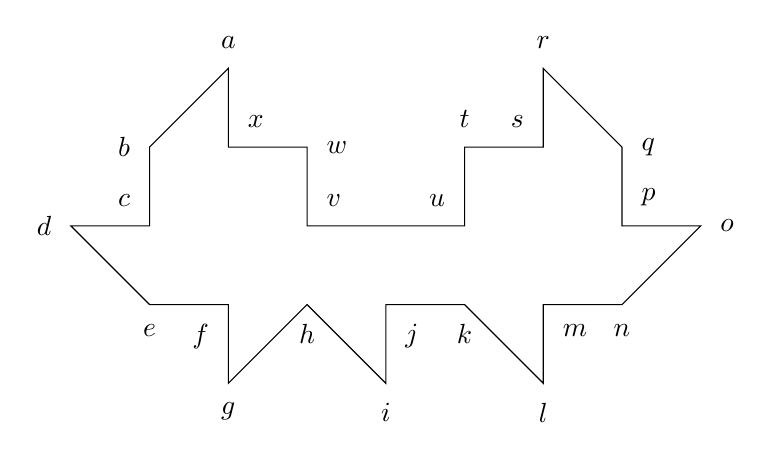
\begin{tikzpicture}
                \draw (-1, -1) node[label=left:$b$] {} -- (0, 0) node[label=north:$a$] {}  -- (0 ,-1) node[label=north east:$x$] {} -- (1, -1) node[label=right:$w$] {} -- (1, -2) node[label=north east:$v$] {} --
                (3,-2) node[label=north west:$u$] {} -- (3,-1) node[label=north:$t$] {} -- (4, -1) node[label=north west:$s$] {} -- (4, 0) node[label=north:$r$] {} -- (5, -1) node[label=right:$q$] {} -- (5, -2) node[label=north east:$p$] {} -- (6,-2) node[label=right:$o$] {} -- (5, -3) node[label=south:$n$] {} -- (4, -3) node[label=south east:$m$] {} -- (4, -4) node[label=south:$l$] {} -- (3, -3) node[label=south:$k$] {} -- (2, -3) node[label=south east:$j$] {} -- (2, -4) node[label=south:$i$] {} -- (1, -3) node[label=south:$h$] {} -- (0, -4) node[label=south:$g$] {} -- (0, -3) node[label=south west:$f$] {} -- (-1, -3) node[label=south:$e$] {} --
                (-2, -2) node[label=left:$d$] {} -- (-1, -2) node[label=north west:$c$] {} -- cycle;
            \end{tikzpicture}
        \end{figure}
        According to the Art Gallery Theorem, how many vertex guards are sufficient to see the entire region? What is the least number of vertex guards actually needed to see the entire region?
    \end{question}
    % Answer 1
    \begin{answer}
        According to the Art Gallery Theorem, the number of vertex guards needed to see the entire region is $\floor*{\frac{24}{3}} = 8$. The least number of vertex guards needed to see the entire region is 2, where the guards are at $x$ and $m$.
    \end{answer}

    % Question 2
    \begin{question}
        Repeat the previous problem for the simple closed polygon below.

        \begin{figure}[H]
            \centering
            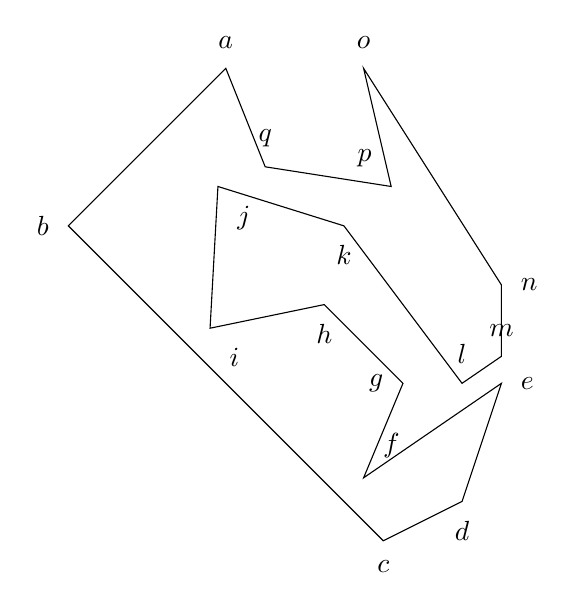
\begin{tikzpicture}
                \draw (0, 0) node[label=north:$a$] {} -- (-2, -2) node[label=left:$b$] {}  --
                (2, -6) node[label=south:$c$] {} --
                (3, -5.5) node[label=south:$d$] {} --
                (3.5, -4) node[label=east:$e$] {} --
                (1.75, -5.2) node[label=north east:$f$] {} -- (2.25, -4) node[label=west:$g$] {} -- (1.25, -3) node[label=south:$h$] {} --
                (-.2, -3.3) node[label=south east:$i$] {} --
                (-.1, -1.5) node[label=south east:$j$] {} --
                (1.5, -2) node[label=south:$k$] {} --
                (3, -4) node[label=north:$l$] {} --
                (3.5, -3.657142857) node[label=north:$m$] {} -- (3.5, -2.75) node[label=east:$n$] {} -- (1.75, 0) node[label=north:$o$] {} -- (2.1, -1.5) node[label=north west:$p$] {} -- (.5, -1.25) node[label=north:$q$] {} -- cycle;
            \end{tikzpicture}
        \end{figure}
    \end{question}
    % Answer 2
    \begin{answer}
        According to the Art Gallery Theorem, the number of vertex guards needed to see the entire region is $\floor*{\frac{17}{3}} = 5$. The least number of vertex guards needed to see the entire region is 3, where the guards are at $f$, $j$, and $p$.
    \end{answer}

    % Question 3
    \begin{question}
        Triangulate one of the two regions above.
    \end{question}
    % Answer 3
    \begin{answer} \
        \begin{figure}[H]
            \centering
            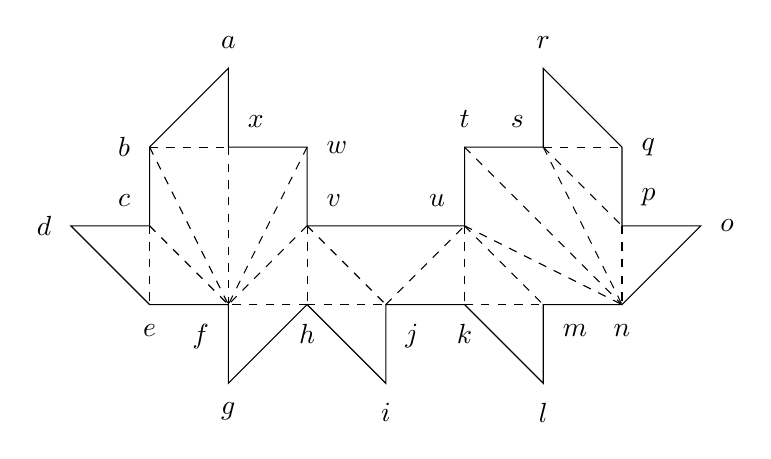
\begin{tikzpicture}
                \draw (-1, -1) node[label=left:$b$] {} -- (0, 0) node[label=north:$a$] {}  -- (0 ,-1) node[label=north east:$x$] {} -- (1, -1) node[label=right:$w$] {} -- (1, -2) node[label=north east:$v$] {} --
                (3,-2) node[label=north west:$u$] {} -- (3,-1) node[label=north:$t$] {} -- (4, -1) node[label=north west:$s$] {} -- (4, 0) node[label=north:$r$] {} -- (5, -1) node[label=right:$q$] {} -- (5, -2) node[label=north east:$p$] {} -- (6,-2) node[label=right:$o$] {} -- (5, -3) node[label=south:$n$] {} -- (4, -3) node[label=south east:$m$] {} -- (4, -4) node[label=south:$l$] {} -- (3, -3) node[label=south:$k$] {} -- (2, -3) node[label=south east:$j$] {} -- (2, -4) node[label=south:$i$] {} -- (1, -3) node[label=south:$h$] {} -- (0, -4) node[label=south:$g$] {} -- (0, -3) node[label=south west:$f$] {} -- (-1, -3) node[label=south:$e$] {} --
                (-2, -2) node[label=left:$d$] {} -- (-1, -2) node[label=north west:$c$] {} -- cycle;

                % c to e
                \draw[dashed] (-1,-2) -- (-1,-3);
                % c to f
                \draw[dashed] (-1,-2) -- (0,-3);
                % b to f
                \draw[dashed] (-1,-1) -- (0,-3);
                % b to x
                \draw[dashed] (-1,-1) -- (0,-1);
                % x to f
                \draw[dashed] (0,-1) -- (0,-3);
                % w to f
                \draw[dashed] (1,-1) -- (0,-3);
                % v to f
                \draw[dashed] (1,-2) -- (0,-3);
                % h to f
                \draw[dashed] (1,-3) -- (0,-3);
                % v to h 
                \draw[dashed] (1,-2) -- (1,-3);
                % h to j
                \draw[dashed] (1,-3) -- (2,-3);
                % v to j
                \draw[dashed] (1,-2) -- (2,-3);
                % j to u
                \draw[dashed] (2,-3) -- (3,-2);
                % u to k
                \draw[dashed] (3,-2) -- (3,-3);
                % u to m
                \draw[dashed] (3,-2) -- (4,-3);
                % k to m
                \draw[dashed] (3,-3) -- (4,-3);
                % u to n
                \draw[dashed] (3,-2) -- (5,-3);
                % p to n
                \draw[dashed] (5,-2) -- (5,-3);
                % t to n
                \draw[dashed] (3,-1) -- (5,-3);
                % s to n
                \draw[dashed] (4,-1) -- (5,-3);
                % s to q
                \draw[dashed] (4,-1) -- (5,-1);
                % s to p
                \draw[dashed] (4,-1) -- (5,-2);
            \end{tikzpicture}
        \end{figure}
    \end{answer}

    % Question 4
    \begin{question}
        Using exactly three colors, color the vertices in your triangulated picture so that each triangle has a vertex of each color.
    \end{question}
    % Answer 4
    \begin{answer} \
        \begin{figure}[H]
            \centering
            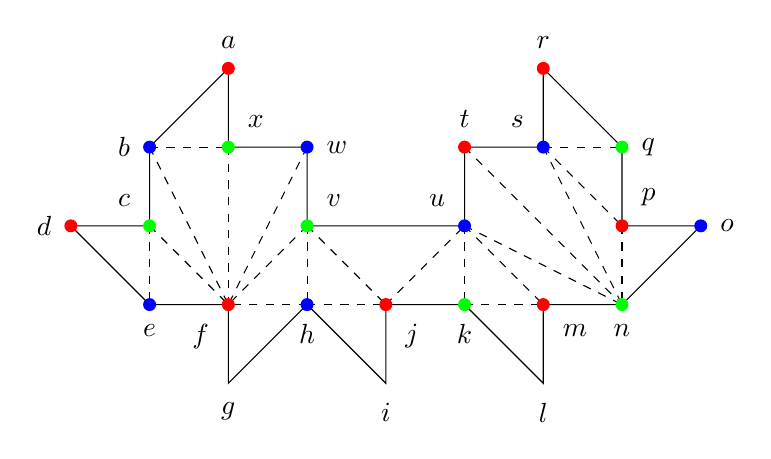
\begin{tikzpicture}
                \draw (-1, -1) node[label=left:$b$] {} -- (0, 0) node[label=north:$a$] {}  -- (0 ,-1) node[label=north east:$x$] {} -- (1, -1) node[label=right:$w$] {} -- (1, -2) node[label=north east:$v$] {} --
                (3,-2) node[label=north west:$u$] {} -- (3,-1) node[label=north:$t$] {} -- (4, -1) node[label=north west:$s$] {} -- (4, 0) node[label=north:$r$] {} -- (5, -1) node[label=right:$q$] {} -- (5, -2) node[label=north east:$p$] {} -- (6,-2) node[label=right:$o$] {} -- (5, -3) node[label=south:$n$] {} -- (4, -3) node[label=south east:$m$] {} -- (4, -4) node[label=south:$l$] {} -- (3, -3) node[label=south:$k$] {} -- (2, -3) node[label=south east:$j$] {} -- (2, -4) node[label=south:$i$] {} -- (1, -3) node[label=south:$h$] {} -- (0, -4) node[label=south:$g$] {} -- (0, -3) node[label=south west:$f$] {} -- (-1, -3) node[label=south:$e$] {} --
                (-2, -2) node[label=left:$d$] {} -- (-1, -2) node[label=north west:$c$] {} -- cycle;

                % c to e
                \draw[dashed] (-1,-2) -- (-1,-3);
                % c to f
                \draw[dashed] (-1,-2) -- (0,-3);
                % b to f
                \draw[dashed] (-1,-1) -- (0,-3);
                % b to x
                \draw[dashed] (-1,-1) -- (0,-1);
                % x to f
                \draw[dashed] (0,-1) -- (0,-3);
                % w to f
                \draw[dashed] (1,-1) -- (0,-3);
                % v to f
                \draw[dashed] (1,-2) -- (0,-3);
                % h to f
                \draw[dashed] (1,-3) -- (0,-3);
                % v to h 
                \draw[dashed] (1,-2) -- (1,-3);
                % h to j
                \draw[dashed] (1,-3) -- (2,-3);
                % v to j
                \draw[dashed] (1,-2) -- (2,-3);
                % j to u
                \draw[dashed] (2,-3) -- (3,-2);
                % u to k
                \draw[dashed] (3,-2) -- (3,-3);
                % u to m
                \draw[dashed] (3,-2) -- (4,-3);
                % k to m
                \draw[dashed] (3,-3) -- (4,-3);
                % u to n
                \draw[dashed] (3,-2) -- (5,-3);
                % p to n
                \draw[dashed] (5,-2) -- (5,-3);
                % t to n
                \draw[dashed] (3,-1) -- (5,-3);
                % s to n
                \draw[dashed] (4,-1) -- (5,-3);
                % s to q
                \draw[dashed] (4,-1) -- (5,-1);
                % s to p
                \draw[dashed] (4,-1) -- (5,-2);

                % Color the vertices
                % a = red
                \filldraw[red] (0, 0) circle (0.075);
                % b = blue
                \filldraw[blue] (-1, -1) circle (0.075);
                % x = green
                \filldraw[green] (0, -1) circle (0.075);
                % f = red
                \filldraw[red] (0, -3) circle (0.075);
                % c = green
                \filldraw[green] (-1, -2) circle (0.075);
                % e = blue
                \filldraw[blue] (-1, -3) circle (0.075);
                % d = red
                \filldraw[red] (-2, -2) circle (0.075);
                % w = blue
                \filldraw[blue] (1, -1) circle (0.075);
                % v= green
                \filldraw[green] (1, -2) circle (0.075);
                % h = blue
                \filldraw[blue] (1, -3) circle (0.075);
                % j = red
                \filldraw[red] (2, -3) circle (0.075);
                % u = blue
                \filldraw[blue] (3, -2) circle (0.075);
                % k = green
                \filldraw[green] (3, -3) circle (0.075);
                % m = red
                \filldraw[red] (4, -3) circle (0.075);
                % n = green
                \filldraw[green] (5, -3) circle (0.075);
                % t = red
                \filldraw[red] (3, -1) circle (0.075);
                % s = blue
                \filldraw[blue] (4, -1) circle (0.075);
                % q = green
                \filldraw[green] (5, -1) circle (0.075);
                % p = red
                \filldraw[red] (5, -2) circle (0.075);
                % r = red
                \filldraw[red] (4, 0) circle (0.075);
                % o = blue
                \filldraw[blue] (6, -2) circle (0.075);
            \end{tikzpicture}
        \end{figure}
    \end{answer}

    % Question 5
    \begin{question}
        Draw a different triangulation of the same region you triangulated in Question 3. Pick two corners on either end of the same exterior wall, and color them with the same colors that you did before. Then color the rest of the vertices so that each triangle has a vertex of each color. Is your new coloring the same as your old coloring?
    \end{question}
    % Answer 5
    \begin{answer} \
        \begin{figure}[H]
            \centering
            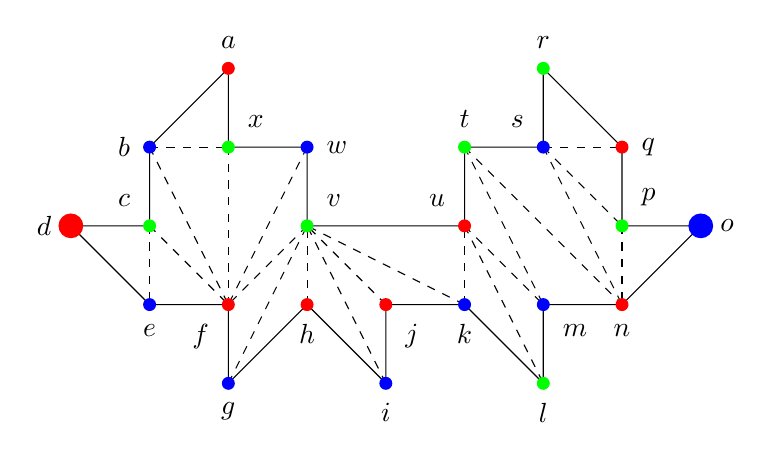
\begin{tikzpicture}
                \draw (-1, -1) node[label=left:$b$] {} -- (0, 0) node[label=north:$a$] {}  -- (0 ,-1) node[label=north east:$x$] {} -- (1, -1) node[label=right:$w$] {} -- (1, -2) node[label=north east:$v$] {} --
                (3,-2) node[label=north west:$u$] {} -- (3,-1) node[label=north:$t$] {} -- (4, -1) node[label=north west:$s$] {} -- (4, 0) node[label=north:$r$] {} -- (5, -1) node[label=right:$q$] {} -- (5, -2) node[label=north east:$p$] {} -- (6,-2) node[label=right:$o$] {} -- (5, -3) node[label=south:$n$] {} -- (4, -3) node[label=south east:$m$] {} -- (4, -4) node[label=south:$l$] {} -- (3, -3) node[label=south:$k$] {} -- (2, -3) node[label=south east:$j$] {} -- (2, -4) node[label=south:$i$] {} -- (1, -3) node[label=south:$h$] {} -- (0, -4) node[label=south:$g$] {} -- (0, -3) node[label=south west:$f$] {} -- (-1, -3) node[label=south:$e$] {} --
                (-2, -2) node[label=left:$d$] {} -- (-1, -2) node[label=north west:$c$] {} -- cycle;

                % c to e
                \draw[dashed] (-1,-2) -- (-1,-3);
                % c to f
                \draw[dashed] (-1,-2) -- (0,-3);
                % b to f
                \draw[dashed] (-1,-1) -- (0,-3);
                % b to x
                \draw[dashed] (-1,-1) -- (0,-1);
                % x to f
                \draw[dashed] (0,-1) -- (0,-3);
                % w to f
                \draw[dashed] (1,-1) -- (0,-3);
                % v to f
                \draw[dashed] (1,-2) -- (0,-3);
                % g to v
                \draw[dashed] (0,-4) -- (1,-2);
                % h to v
                \draw[dashed] (1,-3) -- (1,-2);
                % i to v
                \draw[dashed] (2,-4) -- (1,-2);
                % j to v
                \draw[dashed] (2,-3) -- (1,-2);
                % k to v
                \draw[dashed] (3,-3) -- (1,-2);
                % k to u
                \draw[dashed] (3,-3) -- (3,-2);
                % u to l
                \draw[dashed] (3,-2) -- (4,-4);
                % u to m
                \draw[dashed] (3,-2) -- (4,-3);
                % t to m
                \draw[dashed] (3,-1) -- (4,-3);
                % s to n
                \draw[dashed] (4,-1) -- (5,-3);
                % t to n
                \draw[dashed] (3,-1) -- (5,-3);
                % s to q
                \draw[dashed] (4,-1) -- (5,-1);
                % s to p
                \draw[dashed] (4,-1) -- (5,-2);
                % p to n
                \draw[dashed] (5,-2) -- (5,-3);

                % Color the vertices
                % d = red
                \filldraw[red] (-2, -2) circle (0.15);
                % o = blue
                \filldraw[blue] (6, -2) circle (0.15);
                % c = green
                \filldraw[green] (-1, -2) circle (0.075);
                % e = blue
                \filldraw[blue] (-1, -3) circle (0.075);
                % f = red
                \filldraw[red] (0, -3) circle (0.075);
                % b = blue
                \filldraw[blue] (-1, -1) circle (0.075);
                % x = green
                \filldraw[green] (0, -1) circle (0.075);
                % a = red
                \filldraw[red] (0, 0) circle (0.075);
                % w = blue
                \filldraw[blue] (1, -1) circle (0.075);
                % v = green
                \filldraw[green] (1, -2) circle (0.075);
                % g = blue
                \filldraw[blue] (0, -4) circle (0.075);
                % h = red
                \filldraw[red] (1, -3) circle (0.075);
                % i = blue
                \filldraw[blue] (2, -4) circle (0.075);
                % j = red
                \filldraw[red] (2, -3) circle (0.075);
                % k = blue
                \filldraw[blue] (3, -3) circle (0.075);
                % u = red
                \filldraw[red] (3, -2) circle (0.075);
                % l = green
                \filldraw[green] (4, -4) circle (0.075);
                % t = green
                \filldraw[green] (3, -1) circle (0.075);
                % m = blue
                \filldraw[blue] (4, -3) circle (0.075);
                % n = red
                \filldraw[red] (5, -3) circle (0.075);
                % s = blue
                \filldraw[blue] (4, -1) circle (0.075);
                % p = green
                \filldraw[green] (5, -2) circle (0.075);
                % q = red
                \filldraw[red] (5, -1) circle (0.075);
                % r = green
                \filldraw[green] (4, 0) circle (0.075);
            \end{tikzpicture}
        \end{figure}
        No, the new coloring is not the same as the old coloring.
    \end{answer}

    % Question 6
    \begin{question}
        How many triangles do each of your triangulations contain? How does this number relate to the number of sides in each gallery?
    \end{question}
    % Answer 6
    \begin{answer}
        Both triangulations contain 22 triangles, which is 2 less than the number of sides in the gallery. 
    \end{answer}

    % Question 7
    \begin{question}
        Write down the number 16 as the sum of three different natural numbers, in at least four different ways. In each case, identify a summand which is less than or equal to 5. How does this relate to the proof of the Art Gallery Theorem?
    \end{question}
    % Answer 7
    \begin{answer}
        \begin{align*}
            16 &= \textcolor{red}{1} + \textcolor{red}{5} + 10 \\
            16 &= \textcolor{red}{1} + \textcolor{red}{4} + 11 \\
            16 &= \textcolor{red}{1} + \textcolor{red}{3} + 12 \\
            16 &= \textcolor{red}{1} + \textcolor{red}{2} + 13 \\
        \end{align*}

        This relates to how $\floor*{\frac{16}{3}} = 5$, which gives an upper bound for at least one of the summands. In the Art Gallery Theorem, with a triangulation and each vertex in a triangle is distinct, then at least one of the colors appears $\floor*{\frac{n}{3}}$ times, where $n$ is the number of vertices. In this case, there are 16 vertices, so at least one color appears $\floor*{\frac{16}{3}} = 5$ times. This grants an upper bound for the number of guards needed to guard the gallery.
    \end{answer}

    % Question 8
    \begin{question}
        Consider the following galleries, the first two of which we considered in the lecture videos:
        \begin{figure}[H]
            \centering
            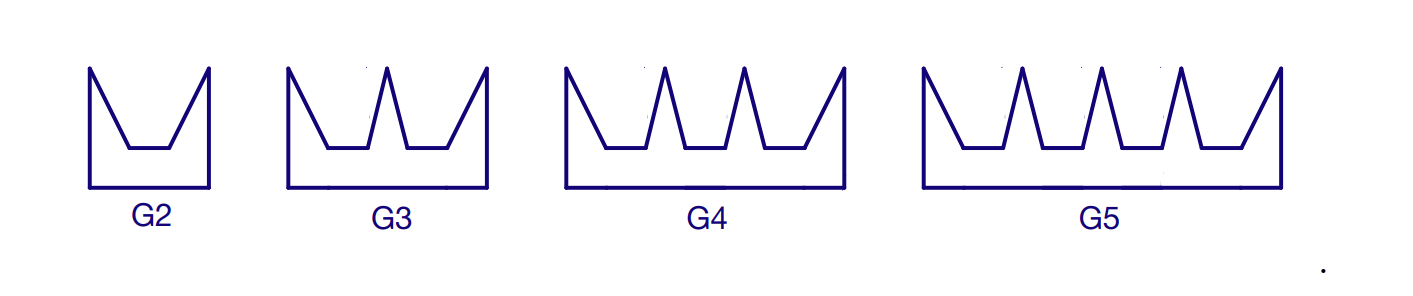
\includegraphics[width=\textwidth]{teeth.png}
        \end{figure}
        If we wished, we could continue the pattern forever, generating infinitely many galleries. Let's let $G_n$ denote the gallery formed this way with $n$ teeth, for $n \geq 2$. How many vertex guards does $G_n$ require? How many vertices does $G_n$ have?
    \end{question}

    % Answer 8
    \begin{answer}
        To watch each tooth, a guard must be placed at each corner where a tooth meets the main gallery. Therefore, $G_n$ requires $n$ vertex guards. 
        \\[12pt]
        $G_n$ has $3n$ vertices, as each tooth has 3 vertices and the main gallery has $n$ teeth.
    \end{answer}
    \section*{Reflection}
    \textbf{Identify at least one wrong or failed idea that turned out to be helpful or enlightening in some way. For instance, that idea might have helped you solve a problem, or it may have been the start of a conversation that improved your understanding more generally. You can list one of your own ideas, or an idea that originated with a classmate. (Please give your classmate credit!)}

    For Question 8, I initially miscounted the number of vertices in $G_n$. I thought that each tooth in the middle had 2 vertices and the left and right most teeth had 3, making a graph of $G_n$ have $6 + 2(n-2) = 2n + 2$ vertices. However, after talking with Larry Huang, I realized that I made a mistake, and that each tooth had 3 vertices.  
\end{document} 
